\documentclass[12pt,a4paper]{amsart}
\usepackage[slovene]{babel}
\usepackage[utf8]{inputenc}
\usepackage{amsmath,amssymb,amsfonts}
\usepackage{url}
\usepackage[dvipsnames,usenames]{color}
\usepackage{graphicx}

\graphicspath{ {./images/} }
\textwidth 15cm
\textheight 24cm
\oddsidemargin.5cm
\evensidemargin.5cm
\topmargin-5mm
\addtolength{\footskip}{10pt}
\pagestyle{plain}
\overfullrule=15pt 
% ukazi za matematicna okolja
\theoremstyle{definition} % tekst napisan pokoncno
\newtheorem{definicija}{Definicija}[section]
\newtheorem{primer}[definicija]{Primer}
\newtheorem{opomba}[definicija]{Opomba}

\renewcommand\endprimer{\hfill$\diamondsuit$}

\theoremstyle{plain} % tekst napisan posevno
\newtheorem{lema}[definicija]{Lema}
\newtheorem{izrek}[definicija]{Izrek}
\newtheorem{trditev}[definicija]{Trditev}
\newtheorem{posledica}[definicija]{Posledica}

% za stevilske mnozice uporabi naslednje simbole
\newcommand{\R}{\mathbb R}
\newcommand{\N}{\mathbb N}
\newcommand{\Z}{\mathbb Z}
\newcommand{\C}{\mathbb C}
\newcommand{\Q}{\mathbb Q}

% ukaz za slovarsko geslo
\newlength{\odstavek}
\setlength{\odstavek}{\parindent}
\newcommand{\geslo}[2]{\noindent\textbf{#1}\hspace*{3mm}\hangindent=\parindent\hangafter=1 #2}


\newcommand{\imeavtorja}{Ana Marija Kravanja}
\newcommand{\naslovdela}{Min-Graph Equipartition Problem with Simulated Annealing}
\newcommand{\letnica}{2019} 

\begin{document}

% od tod do povzetka ne spreminjaj nicesar
\thispagestyle{empty}
\noindent{\large
UNIVERZA V LJUBLJANI\\[1mm]
FAKULTETA ZA MATEMATIKO IN FIZIKO\\[5mm]}
\vfill

\begin{center}{\large
{\bf \naslovdela}\\[10mm]
Ana Marija Kravanja, Urška Jeranko, Oskar Kregar}\\[1cm]

\end{center}
\vfill

\noindent{\large
Ljubljana, \letnica}
\pagebreak


\section{Osnovno o projektu}
Reševali bomo problem deljenja grafa. Graf želimo razdeliti na dva priližno enaka dela pri čemer je med njima čim manj povezav. Najti tako delitev ni preprosto. Problem postane še težji, če moramo iskati med zelo veliko rešitvami da najdemo pravo. Reševali ga bomo s požrešno metodo in metodo simuliranega izničenja. Rešitve teh metod bomo primerjali med sabo in jih preizkusili na več različnih grafih pri različnih parametrih. 

\section{Požrešna metoda}
Požrešna metoda je strategija pri kateri optimalno rešitev izberemo na vsakem koraku posebej s ciljem da bi našli globalno optimalno rešitev. Problem metode je, da na vsakem koraku izberemo najboljšo rešitev, kar nas pripelje do lokalnega optimuma, ne pa nujno globalnega. Možno je tudi, da nas privede celo do najslabšega globalnega rezultata. \\

Naj bo $G=(V,E)$ enostaven graf, pri čemer je $V$ množica vozlišč in $E$ množica povezav. Naj bo število vozlišč enako $n$. Definirajmo delitev grafa na dve množici X in Y, pri čemer je $|X| = \lceil \frac{n}{2} \rceil$. Širina bisekcije je najmanjše število povezav med $X$ in $Y$ med vsemi možnimi delitvami. 

\begin{definicija}
Naj bo $G=(V,E)$ enostaven graf in $X,Y \subseteq V$, tako da je $X \cap Y = \emptyset$ in $X \cup Y =V$.
\begin{itemize}
\item Za $x \in X$ označimo $I(x)$ notranja vrednost, to je šteilo povezav $(x,z) \in E;z\in X \backslash \{x\}$ . Analogno definiramo $I(y)$ za $y \in Y$.
\item Za $x \in X$ označimo $O(x)$ zunanja vrednost, to je šteilo povezav $(x,z) \in E;z\in Y $ . Analogno definiramo $O(y)$ za $y \in Y$.
\item Za $x \in X, y \in Y$ naj bo $\omega(x,y) := \begin{cases} 1,&\text{if} (x,y) \in E\\ 
0, &\text{sicer}\end{cases} $.
\item Za $x \in X, y \in Y$ naj bo $S(x,y):= O(x)-I(x)+O(y)-I(y)-2\omega(x,y)$.
\end{itemize}
\end{definicija}

\subsection{Algoritem požrešne metode}
Začnemo z naključno delitvijo vozlišč grafa. Algoritem zamenja dve vozlišči na različnih straneh, če nam to predstavlja boljšo bisekcijo in se ustavi, če to ni več možno. Pri menjavi notranje vrednosti postanejo zunanje in obratno, zato dobimo izboljšano bisekcijo le če je $S(x,y)>0$.
\subsubsection{Algoritem 1} 
Vhodni podatki: Graf $G=(V,E), |V|=n$.
\begin{enumerate}
\item Izberemo neključno delitev $(X,Y)$.
\item Izberemo $x\in X, y\in Y$, tako da je $S(x,y)>0$.
\item Zamenjamo vozlišči $x$ in $y$.
\item Ponavljamo 2. in 3. korak dokler ne obstajata več $x\in X, y\in Y$, da je $S(x,y)>0$.
\end{enumerate}
Izhodni podatki: delitev $(X,Y)$.

\section{Metoda simulacijskega izničenja}
Metoda simulacijskega izničenja je verjetnostna strategija za aproksimacijo globalnega optimuma dane funkcije. Razlika od požrešne metode je to, da na vsakem koraku lahko izberemo tudi slabšo rešitev z neko verjetnostjo, vendar nas na koncu privede do globalnega optimuma.  
Metoda ej dobila ime zaradi procesa toplotne obdelave kovin. Ta vsebuje segrevanje in ohlajanje materiala da spremenimo fizikalne lastnosti v notranji strukturi. Ko se kovina ohladi postane njena nova dtruktura fiksna, kar povzroči da kovina pridobi določene lastnosti. V simulacijskem izničenju ohranimo temperaturno spremenljivko, ki simulira ogrevalni proces. Na začetku ga nastavimo višje, da je proces hlajenja daljši in se algoritem dlje časa izvaja. Algoritem bo namreč pogosteje sprejemal rešitve, ki so slabše od naše trenutne rešitve. Vendar se algoritem čez čas osredotoči na območje iskalnega prostora, v katerem upamo, da je mogoče najti optimalno rešitve. Algoritem je zelo učinkovit pri iskanju bližine optimalnih problemov rešitvi pri obravnavanju velikih problemov, ki vsebujejo številne lokalne optimalnosti. 

\subsection{Algoritem metode simulacijskega izničenja}
Graf si definiramo analogno kot pri požrešni metodi. Če je $S(x,y)>0$ zamenjamo vozlišči, če pa je $S(x,y)<0$ pa z verjetnostjo $$P(x,y,t) = e^{\frac{S(x,y)}{t}}; t\ge 0$$.

\subsubsection{Algoritem 2}
S $Q(Z)$ je označena funkcija, ki množici Z priredi neko kvaliteto, torej če je $Q(Z) >Q(R)$ pomeni da je množica Z bolj ugodna za nadaljno obravnavo.
Za funkcijo $Q$ smo si v našem primeru izbrali $S(x,y)$, ki je definiran enako kot pri prejšni požrešni metodi. Torej če je $S(x,y)$ funkcija,kjer smo v množici $R$ zamenjali x in y in $S(a,b)$ množica $Z$ kjer jih nismo zamenjali in velja da je $S(x,y) > S(a,b)$, potem z določeno verjetnostjo zamenjamo $R$ z $Z$. 
\begin{enumerate}
\item t= temperatura z visoko vrednostjo
\item Z= začetna delitev grafa na množici X in Y 
\item N= Z  naj predstavlja trenutno najboljšo rešitev
\item ponovi dokler je N najboljša rešitev, nam je zmanjkalo časa ali pa je $t \leq 0$
\item 			R=delitev, kjer zamenjamo $x$ in $y$
\item 			če je $Q(R)>Q(Z)$ ali naključno število med 0 in 1 manjše od $P(x,y,t)$, potem je $S=R$
\item 			zmanjšamo t
\item 			če je $Q(Z)>Q(N)$ 
\item 				$N=Z$
\item vrni $N$		
\end{enumerate}


\section{Primeri}
Poglejmo si nekaj primerov delitve grafov. 

\begin{figure}[h]
    \centering
    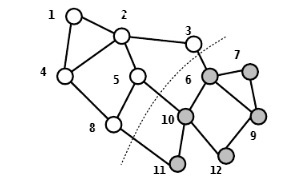
\includegraphics{prvi_graf} 
    \caption{primer grafa na 12 točkah}
    \label{fig:1_graf}
\end{figure}

\begin{figure}[h]
    \centering
    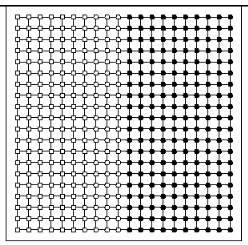
\includegraphics{drugi_graf} 
    \caption{primer grafa na 400 točkah, prikazana je optimalna rešitev}
    \label{fig:2_graf}
\end{figure}

\begin{figure}[h]
    \centering
    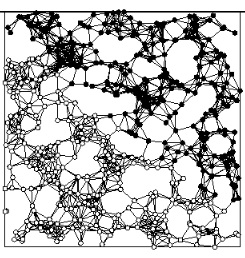
\includegraphics{tretji_graf} 
    \caption{Johnsonsov geometrični graf}
    \label{fig:3_graf}
\end{figure}


\end{document}
